\documentclass[notitlepage, 11pt]{article}

\usepackage[a4paper, top=3cm, bottom=4cm, left=3.75cm, right=3.75cm, head=1.2cm, foot=2cm]{geometry}
\usepackage{cite}
\usepackage{dirtytalk}
\usepackage{mathtools}
\usepackage{enumitem}
\usepackage{graphicx}
\usepackage{caption}
\usepackage{subcaption}
\usepackage{float}
\usepackage{listings}
\usepackage{xcolor}
\usepackage[hidelinks]{hyperref}
\usepackage[toc,page]{appendix}

\lstset{
  frame=single,
  breaklines=true,
  showstringspaces=false,
  postbreak=\raisebox{0ex}[0ex][0ex]{\ensuremath{\color{red}\hookrightarrow\space}}
}

\DeclarePairedDelimiter\abs{\lvert}{\rvert}%
\DeclarePairedDelimiter\norm{\lVert}{\rVert}%

% Swap the definition of \abs* and \norm*, so that \abs
% and \norm resizes the size of the brackets, and the
% starred version does not.
\makeatletter
\let\oldabs\abs
\def\abs{\@ifstar{\oldabs}{\oldabs*}}
%
\let\oldnorm\norm
\def\norm{\@ifstar{\oldnorm}{\oldnorm*}}
\makeatother

\title{IMT4202 Assignment 3}
\author{Magnus Bjerke Vik}
\date{\today}

\begin{document}

\maketitle

\section*{1.}

Both matrices \(W^a_8\) and \(W^a_4\) was found using the Python code in Listing~\ref{lst:find-dwt-mat}.
They are calculated in Listing~\ref{lst:w4-w8} and displayed in Listing~\ref{lst:w4} and Listing~\ref{lst:w8}.
Note that the precision of the numbers have been lowered to fit the page width.
The code in Listing~\ref{lst:find-dwt-mat} loops through half of the rows in the matrix, and for each row inserts the low-pass filter to the upper part of the matrix and the high-pass filter to the lower part of the matrix.

The Haar DWT of the vector, x, is computed in Listing~\ref{lst:x-dwt}.
The resulting DWT is as follows: \([2.83, 3.54, 2.12, 4.24, -1.41, 0.71, -0.71, 0.0]\)

\lstinputlisting[
  language=Python,
  firstline=10,
  lastline=23,
  label={lst:find-dwt-mat},
  caption={Finding the dwt matrix for a wavelet}]
  {code.py}

\lstinputlisting[
  language=Python,
  firstline=55,
  lastline=56,
  label={lst:w4-w8},
  caption={Finding W4 and W8}]
  {code.py}

\begin{lstlisting}[
  label={lst:w4},
  caption={W4}]
[ 0.71  0.    0.    0.71]
[ 0.    0.71  0.71  0.  ]
[ 0.71  0.    0.   -0.71]
[ 0.   -0.71  0.71  0.  ]
\end{lstlisting}

\begin{lstlisting}[
  label={lst:w8},
  caption={W8}]
[ 0.71  0.    0.    0.    0.    0.    0.    0.71]
[ 0.    0.71  0.71  0.    0.    0.    0.    0.  ]
[ 0.    0.    0.    0.71  0.71  0.    0.    0.  ]
[ 0.    0.    0.    0.    0.    0.71  0.71  0.  ]
[ 0.71  0.    0.    0.    0.    0.    0.   -0.71]
[ 0.   -0.71  0.71  0.    0.    0.    0.    0.  ]
[ 0.    0.    0.   -0.71  0.71  0.    0.    0.  ]
[ 0.    0.    0.    0.    0.   -0.71  0.71  0.  ]
\end{lstlisting}

\lstinputlisting[
  language=Python,
  firstline=57,
  lastline=58,
  label={lst:x-dwt},
  caption={Computing Harr DWT of x}]
  {code.py}

\section*{2}

To create \(\mathcal{W}^a_2\) from \(W^a_8\) and \(W^a_4\), a function that can create a matrix with any number of levels is used.
The function is found in Listing~\ref{lst:multi-dwt}.
For each level going backwards it creates a matrix for that level and multiplies it with the previous level's matrix, such that the resulting matrix will be a multiplication of all the levels' matrices.

The function is used in Listing~\ref{lst:x-muldwt} to compute the 2-level Harr DWT of x.
The matrix is displayed in Listing~\ref{lst:multi-dwt-mat}, and the results are as follows:\\
\([5.0, 4.0, -1.0, -1.0, -1.41, 0.71, -0.71, 0.0]\)

The result has been checked by manually computing the two-level Haar DWT with the code in Listing~\ref{lst:mul-dwt-man}.
The results were exactly the same.

\lstinputlisting[
  language=Python,
  firstline=26,
  lastline=51,
  label={lst:multi-dwt},
  caption={Function to create multilevel DWT matrix}]
  {code.py}

\lstinputlisting[
  language=Python,
  firstline=82,
  lastline=84,
  label={lst:x-muldwt},
  caption={Computing 2-level DWT of x}]
  {code.py}

\begin{lstlisting}[
  label={lst:multi-dwt-mat},
  caption={2-level Haar DWT matrix}]
[ 0.5   0.    0.    0.    0.    0.5   0.5   0.5 ]
[ 0.    0.5   0.5   0.5   0.5   0.    0.    0.  ]
[ 0.5   0.    0.    0.    0.   -0.5  -0.5   0.5 ]
[ 0.   -0.5  -0.5   0.5   0.5   0.    0.    0.  ]
[ 0.71  0.    0.    0.    0.    0.    0.   -0.71]
[ 0.   -0.71  0.71  0.    0.    0.    0.    0.  ]
[ 0.    0.    0.   -0.71  0.71  0.    0.    0.  ]
[ 0.    0.    0.    0.    0.   -0.71  0.71  0.  ]
\end{lstlisting}

\lstinputlisting[
  language=Python,
  firstline=86,
  lastline=95,
  label={lst:mul-dwt-man},
  caption={Computing 2-level DWT of x manually}]
  {code.py}

\section*{3.}

The code used for this task is designed so that it can be repeated as specified in Task 4 and 5.
This means that the code is more complex than necessary for this task, and that parts of Task 4 and 5 will be covered here.

As shown in Listing~\ref{lst:img-dwt}, the image is first opened, converted to greyscale and transformed to a DWT representation.
Then it has all of its details set to 0 by going through the DWT array (approximation is the first index, and for each level there is a tuple of size 3) in Listing~\ref{lst:img-dwt-zero}.
The DWT is then inverse transformed to the image and saved to a file in Listing~\ref{lst:img-idwt}.
The result can be seen in Figure~\ref{fig:task3}.

To visualize the DWT, the approximation (first index) plus the details for each level are stitched together in Listing~\ref{lst:dwt-vis}.
This happens before the details are set to 0.
The upper left part (approximation plus previous) is merged with the lower left part (horizontal detail) vertically.
The upper right part (vertical detail) is merged with the lower right part (diagonal detail) vertically.
Both of these are then merged horizontally to form the full visualization for that level.
This is then repeated for each level to form the multilevel visualization.
Note that some wavelets will produce details of lower resolution, and thus will have to be resized to the proper size.

The visualized version of the DWT for this task can be found in Figure~\ref{fig:task3}.

\lstinputlisting[
  language=Python,
  firstline=118,
  lastline=121,
  label={lst:img-dwt},
  caption={DWT of image}]
  {code.py}

\lstinputlisting[
  language=Python,
  firstline=149,
  lastline=151,
  label={lst:img-dwt-zero},
  caption={Setting details to zero}]
  {code.py}

\lstinputlisting[
  language=Python,
  firstline=153,
  lastline=155,
  label={lst:img-idwt},
  caption={Recovering and saving the image}]
  {code.py}

\lstinputlisting[
  language=Python,
  firstline=123,
  lastline=147,
  label={lst:dwt-vis},
  caption={Visualizing the DWT of the image}]
  {code.py}

\begin{figure}[H]
  \centering
  \begin{subfigure}[t]{0.5\textwidth}
    \centering
    \includegraphics[width=0.9\textwidth]{img/lena_1_haar}
    \caption{Image with details removed}
  \end{subfigure}%
  ~
  \begin{subfigure}[t]{0.5\textwidth}
    \centering
    \includegraphics[width=0.9\textwidth]{img/lena_1_haar_dwt}
    \caption{Image DWT}
  \end{subfigure}%
  \caption{Lena image without details and DWT}
  \label{fig:task3}
\end{figure}

%\subsection*{B.}

%Figure~\ref{fig:1b} displays the power spectrum of y.
%As seen from the figure, the peaks correspond to the frequencies in the signal.
%The code for computing the DFT and plotting the spectrum is shown in Listing~\ref{lst:1b}.

%\begin{figure}[H]
%  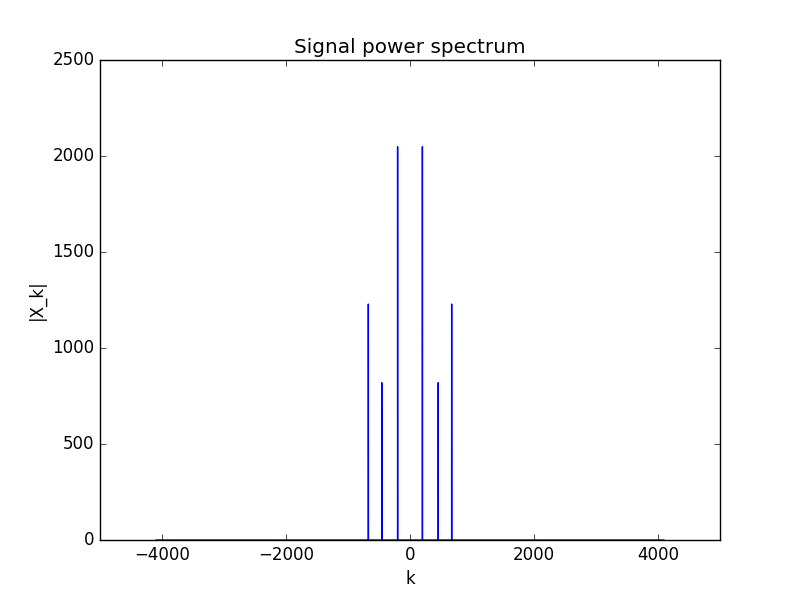
\includegraphics[width=\textwidth]{1b}
%  \caption{Signal y power spectrum}
%  \label{fig:1b}
%\end{figure}

%\lstinputlisting[
%  language=Python,
%  firstline=28,
%  lastline=35,
%  label={lst:1b},
%  caption={Signal y power spectrum}]
%  {code.py}

%\subsection*{C.}

%Listing~\ref{lst:filter-dft} creates the filter DFT as defined in the task.
%Figure~\ref{fig:1c-power} displays the power spectrum of this filter, plotted by Listing~\ref{lst:filter-power}.
%The filter DFT is inverse DFT transformed in Listing~\ref{lst:filter-idft} to get the filter which is plotted in Figure~\ref{fig:1c-filter} by Listing~\ref{lst:filter-plot}.
%All the components of the filter are nonzero, as calulated by Listing~\ref{lst:nonzero}.

%\lstinputlisting[
%  language=Python,
%  firstline=37,
%  lastline=43,
%  label={lst:filter-dft},
%  caption={Filter DFT (H)}]
%  {code.py}

%\lstinputlisting[
%  language=Python,
%  firstline=46,
%  lastline=51,
%  label={lst:filter-power},
%  caption={H power spectrum}]
%  {code.py}

%\begin{figure}[H]
%  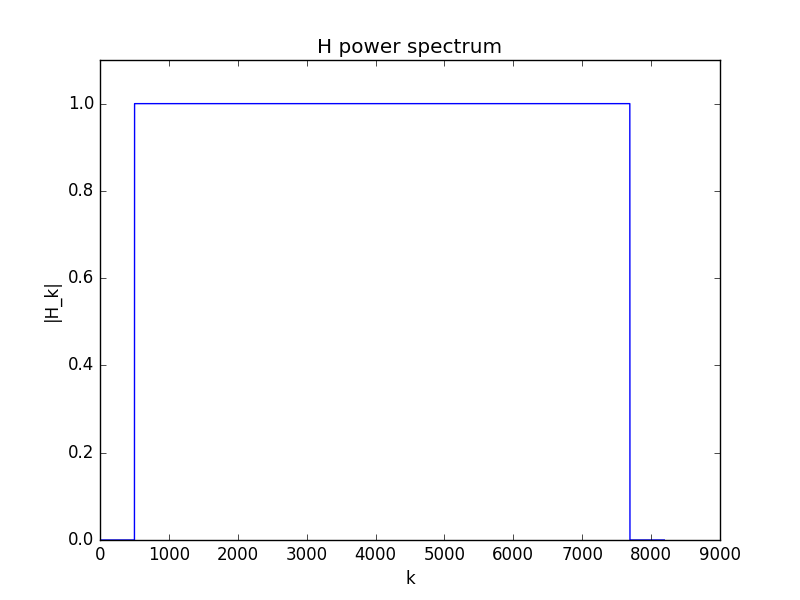
\includegraphics[width=\textwidth]{1c_power}
%  \caption{H power spectrum}
%  \label{fig:1c-power}
%\end{figure}

%\lstinputlisting[
%  language=Python,
%  firstline=44,
%  lastline=44,
%  label={lst:filter-idft},
%  caption={H inverse DFT}]
%  {code.py}

%\lstinputlisting[
%  language=Python,
%  firstline=53,
%  lastline=58,
%  label={lst:filter-plot},
%  caption={h filter signal}]
%  {code.py}

%\begin{figure}[H]
%  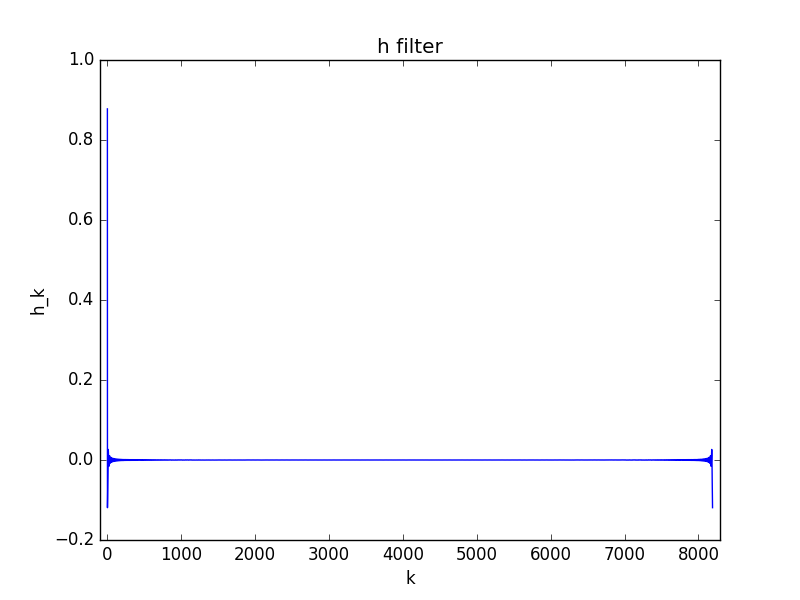
\includegraphics[width=\textwidth]{1c_signal}
%  \caption{h filter signal}
%  \label{fig:1c-filter}
%\end{figure}

%\lstinputlisting[
%  language=Python,
%  firstline=60,
%  lastline=61,
%  label={lst:nonzero},
%  caption={Nonzero count of signal}]
%  {code.py}

%\subsection*{D.}

%The signal y was filtered with h by conjugating y and h in Listing~\ref{lst:conj}, then written to an audio file in Listing~\ref{lst:conj-write}.
%One could clearly hear only the highest frequency.
%Figure~\ref{fig:filtered} displays the power spectrum of the filtered signal.
%It was created by the code in Listing~\ref{lst:filtered-plot}.
%The spectrum shows that only one frequency remains.

%\lstinputlisting[
%  language=Python,
%  firstline=63,
%  lastline=63,
%  label={lst:conj},
%  caption={Filtering signal y with filter h by conjugation}]
%  {code.py}

%\lstinputlisting[
%  language=Python,
%  firstline=64,
%  lastline=64,
%  label={lst:conj-write},
%  caption={Writing the filtered signal}]
%  {code.py}

%\lstinputlisting[
%  language=Python,
%  firstline=66,
%  lastline=70,
%  label={lst:filtered-plot},
%  caption={Plotting the power spectrum of the filtered signal}]
%  {code.py}

%\begin{figure}[H]
%  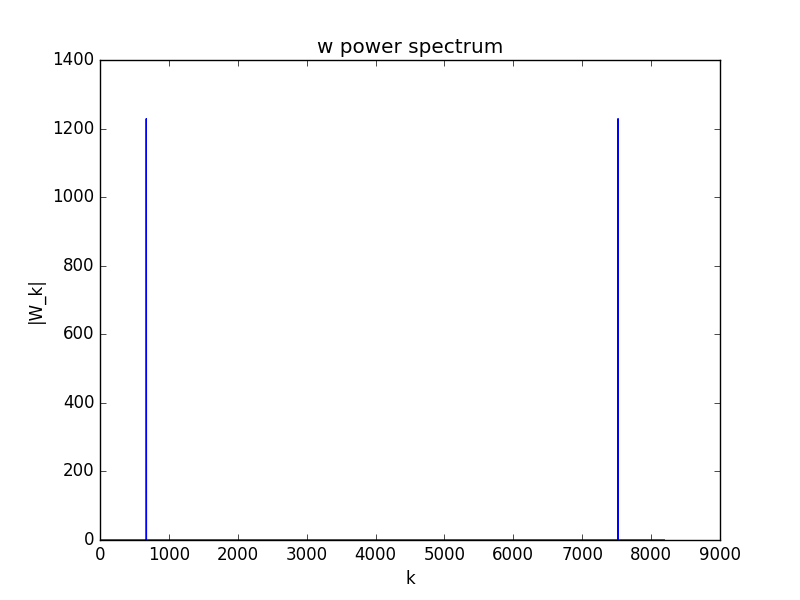
\includegraphics[width=\textwidth]{1d}
%  \caption{Power spectrum of filtered signal}
%  \label{fig:filtered}
%\end{figure}

%\section*{2.}

%\subsection*{A.}

%The signal is sampled, transformed by DFT and plotted in Listing~\ref{lst:2a}.
%The plot is seen in Figure~\ref{fig:2a}.
%From the plot one can clearly see two frequencies which should be 137 and 147.
%The first frequency is much stronger than the second, which matches with the amplitudes in the signal.

%\lstinputlisting[
%  language=Python,
%  firstline=74,
%  lastline=90,
%  label={lst:2a},
%  caption={Signal sampling and DFT magnitude plot}]
%  {code.py}

%\begin{figure}[H]
%  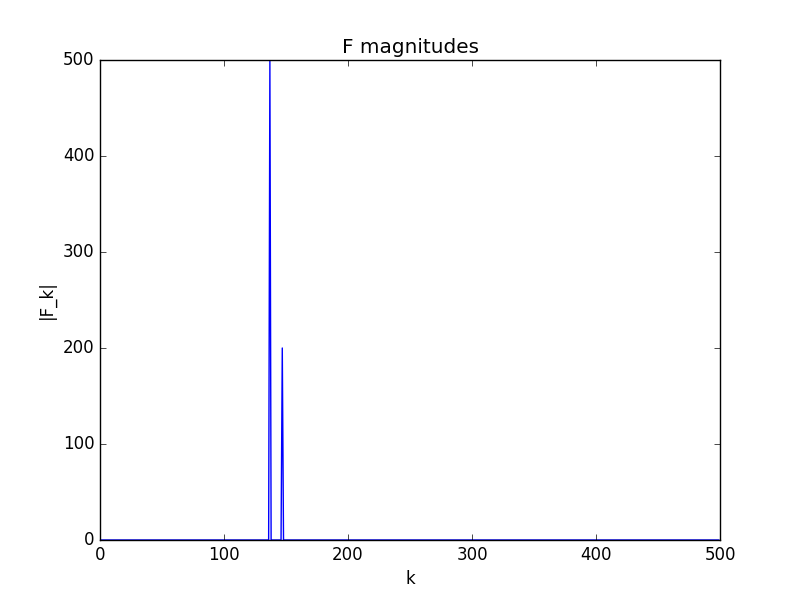
\includegraphics[width=\textwidth]{2a}
%  \caption{DFT magnitudes of signal}
%  \label{fig:2a}
%\end{figure}

%\subsection*{B.}

%Listing~\ref{lst:window} constructs a windowed version of the signal with a size of 200 and plots the magnitudes of the first 100 components of the DFT.
%The plot can be seen in Figure~\ref{fig:window}.
%The two frequencies still have distinguishable spikes, but they are much wider than earlier.

%\lstinputlisting[
%  language=Python,
%  firstline=92,
%  lastline=99,
%  label={lst:window},
%  caption={Window DFT and plot}]
%  {code.py}

%\begin{figure}[H]
%  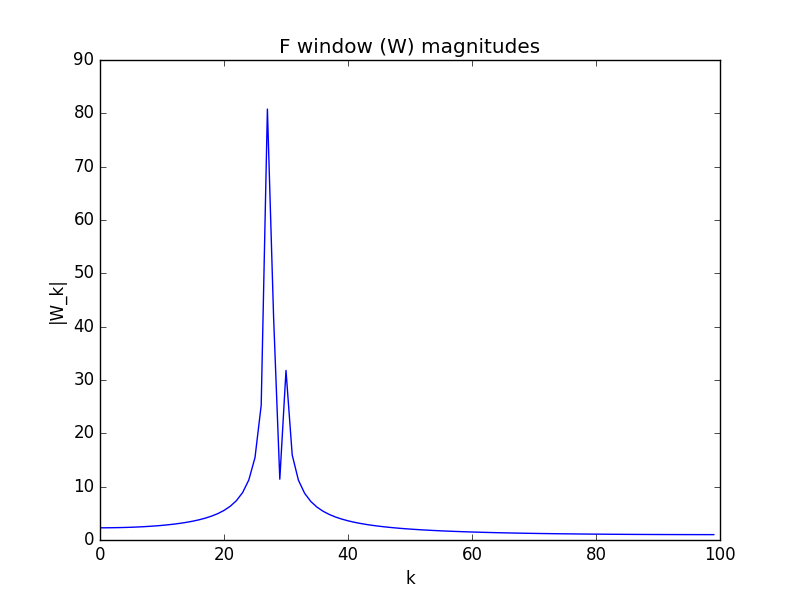
\includegraphics[width=\textwidth]{2b}
%  \caption{Windowed signal magnitude plot}
%  \label{fig:window}
%\end{figure}
 % includes latex files from the same directory

\begin{appendices}
	\section{All Source Code}
\lstinputlisting[
  language=Python,
  caption={All source code}]
  {code.py}

\end{appendices}

\end{document}

% vim: set ts=2 sw=2 expandtab:
